\documentclass[a4paper,pdftex,DIV18,parskip=half+]{scrartcl}

\usepackage[utf8]{inputenc}
\usepackage{default}
\usepackage[T1]{fontenc}

% \usepackage{ngerman}
\usepackage{amssymb, amsmath}
\usepackage{hyperref}
\usepackage{eurosym}
% quellcode listings
\usepackage{color}
\usepackage{listings} % Quellcode benutzte
% \usepackage{bold-extra}
% \usepackage{lmodern}
% \usepackage{courier}
\usepackage{textcomp}

\lstset{
  language=C++,
  morekeywords={QObject,QKDProcessor,QList,QPair,Index,IndexBoolList,IndexList,%
                BoolList,IndexBoolPair,IndexBoolPairList,Measurement,%
                Measurements,emit,QString},
  basicstyle=\scriptsize,
  keywordstyle=\bfseries,
  commentstyle=\itshape\color{green!70!black},
  % stringstyle=\itshape\color{red!70!black},
  stringstyle=\color{red!70!black},
  identifierstyle=\ttfamily,
  numbers=left,
  numberstyle=\tiny,
  stepnumber=1,
  tabsize=4,
  showspaces=false,
  showstringspaces=false,
  breaklines=true,
  frame=single, % shadowbox
%   columns=fixed,
  columns=fullflexible,
  captionpos=t,
  extendedchars=\true,
  inputencoding=utf8,
  backgroundcolor=\color{white!95!black},
  postbreak = \raisebox{0ex}[0ex][0ex]{\ensuremath{\hookrightarrow}},
  rulecolor=\color{black}
}

\usepackage{tikz}


\usepackage{siunitx}
\sisetup{
  separate-uncertainty = true,
  multi-part-units = brackets,
  open-bracket = (,
  close-bracket = ),
  exponent-product = \cdot,
  add-decimal-zero = true,
  add-integer-zero = true,
  per-mode         =   reciprocal,
%   prefixes-as-symbols = true,
  output-decimal-marker = {,},
  table-figures-uncertainty = 1,
  load-configurations=abbreviations,
  sticky-per
}
\title{Documentation to privacy-amplification \newline – INTERNAL DRAFT –}
\author{Robert Riemann}

\begin{document}
\maketitle
% \pagestyle{plain}

\begin{figure}[htb!]
  \centering
  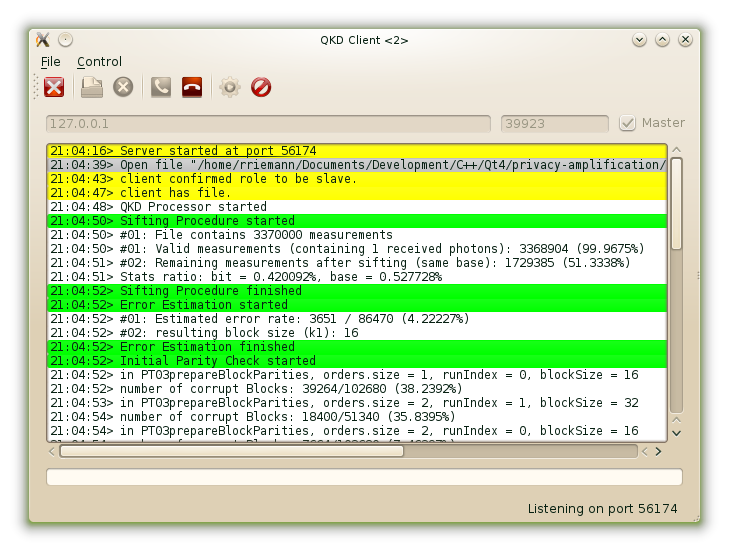
\includegraphics[width=0.8\textwidth,keepaspectratio=true]{./screenshot.png}
  % screenshot.png: 729x551 pixel, 96dpi, 19.29x14.58 cm, bb=0 0 547 413
  \caption{Screenshot of the QKD Client in Alice-mode}
\end{figure}



\section*{Note on Qt (Framework)}

This software uses the cross-platform C++ framework Qt (pronounced like “cute”, LPGL licensed). Hence there
are some C++ language extensions.

\begin{itemize}
  \item Macros starting with \texttt{Q\_}
  \item additional keywords like \texttt{foreach} and \texttt{emit}
\end{itemize}

\texttt{emit} is part of the Signals/Slots mechanism\footnote{%
\url{http://qt-project.org/doc/qt-4.8/signalsandslots.html}} and is used to
trigger a so called Signal. Other objects, which are listening to that \emph{Signal}
might react by processing their connected \emph{Slots}. The code execution doesn't
take place immediately, but anytime later and is triggered by the global event loop.

This means that emitting a signal doesn't cause any delay, even if connected slots
rely on network.

Qt comes with a comprehensive documentation which is also available online at: \\
\url{http://qt-project.org/doc/qt-4.8/}


\section*{Detailed Description}



The most important stuff is in \texttt{QKDProcessor::incomingData(quint8
type, QVariant data)}, which is defined in \texttt{qkdprocessor.cpp}.

On loading this application, one \texttt{QKDProcessor} Object is instanciated.
The \texttt{Mainwindow} Object starts the protocol by calling
\texttt{QKDProcessor::start(bool isMaster)} after is has been made sure,
that a file was loaded and the measurements were assigned by
\texttt{QKDProcessor::setMeasurements(Measurements \*measurements)}.

Measurements are usually allocated onto the heap (using \texttt{new}) and
consists of 3 boolean properties:
\begin{description}
  \item[valid] \hfill \\ a flag which marks this measurement as valid. This is used on
               Bob's side to mark measurements with more than two registrated
               photons as invalid.
  \item[base]  \hfill \\ a flag to save the state accordingly to the chosen base out of 2.
  \item[bit]   \hfill \\ a flag to save the bit which was transfered. These bits constitutes
               later on our cryptographic key.
\end{description}

The list of pointers to all measurements is managed by a \texttt{QList} objects,
which is itself also allocated onto the heap to make it easy to pass these
measurements between a file and our \texttt{QKDProcessor} object.

\begin{lstlisting}[caption={extract of measurement.h}]
struct Measurement
{
    Measurement(bool base, bool bit, bool valid = 1) : base(base), bit(bit), valid(valid) {}
    explicit Measurement() : base(0), bit(0), valid(1) {}
    Measurement &operator=(const Measurement &other)
    {base = other.base; bit = other.bit; valid = other.valid; return *this;}

    bool base;
    bool bit;
    bool valid;
};
typedef QList<Measurement*> Measurements;
\end{lstlisting}


After the processing has started, the
\texttt{QKDProcessor::incomingData(quint8 type, QVariant data)} is called
alternately by Alice, also known as \texttt{isMaster} (\texttt{bool}), and
Bob, respectively \texttt{!isMaster}.

\subsection*{Important Variables}

To keep the variable declaration right next to the code, most variables used
to implement the protocol are not declared as member variables of
\texttt{QKDProcessor}, but as \texttt{static} local variables right on top of
\texttt{incomingData} method.

\begin{description}
  \item[\texttt{qreal} error] \hfill \\ Error probability.
        The error probabilities estimated by comparing \SI{0.05}{\percent} of
        all bits. These bits were deleted immediately afterward. 
  \item[\texttt{quint16} k1] \hfill \\ Initial block size calculated by
       \texttt{calculateInitialBlockSize(qreal errorProbability)}.
  \item[\texttt{quint8} runCount] \hfill \\ This constant integer setups the limit of
        individual reorderings of all data. Each consecutive reordering doubles
        the block size starting with \texttt{k1}.
  \item[\texttt{quint8} runIndex] \hfill \\ Run index counts towards
        \texttt{runCount}.
  \item[\texttt{quint16} blockSize] \hfill \\ The actual block size can be
        determined using \texttt{runCount} and \texttt{k1}.
  \item[\texttt{Index} blockCount] The total count of blocks depends on the
        total count of measurements as well as the current \texttt{blockSize}.
        To overcome issues with incomplete blocks, the overlap gets deleted
        initially.
\end{description}

\subsection*{Program Run}

\begin{enumerate}
  \item measurement data get loaded using \texttt{setMeasurements} method
  \item protocol gets started using \texttt{start} method
  \item Alice asks Bob to send an \texttt{IndexList} of received photons (\texttt{PT01sendReceivedList}).
  \item Bob answers by sending a list of indexes with his valid measurement including with his chosen base.
  \item Alice calculated the remaining measurements taking only measurements with same base into account.
  \item Alice sends a list of indexes of his remaining measurement to Bob. (\texttt{PT01sendRemainingList})
  \item Bob receives this list, reports his to Alice and both do the sifting using \texttt{siftMeasurements}.
  \item Alice requires Bob to send back a specific count of bits (taken from the
        last measurements) to estimate the error probability (\texttt{PT02errorEstimationSendSample}).
  \item Bob responds by sending this amount of bits and deleting the appropriate
        measurements immediately.
  \item Alice compares the bits to calculate the error probability
        (\texttt{error}) and reports the absolute count of errors back to Bob
        who calculates the same error on his own (\texttt{PT02errorEstimationReport}).
  \item Both parties calculate the inital block size \texttt{k1} which depends
        \texttt{error}. Afterwards the parities are calculated at the same time.
        The initial bit order is set up to be chronological (\textit{about to change soon!}). 
  \item Alice sends Bob the order to report his blocks with wrong parities
        (corrupt block) given Alices parities (\texttt{PT04reportBlockParities}).
        
        As the block size is known to both (first \texttt{blockSize},
        \texttt{binaryBlockSize} while doing BINARY), it is sufficient to only
        refer to the index of the first measurement of the corrupt block given
        the ordering related to the current \texttt{runIndex}/\texttt{blockSize}.
  \item Bob does so and Alice receives the (maybe empty) list of corrupt blocks.
        Alice has to decide what has to be done next:
        \begin{enumerate}
          \item start or continue BINARY
          \item create a new random ordering of all measurements and send it to
                Bob to enter the next level (\texttt{runIndex})
          \item go back to first level (\texttt{runIndex}) to correct new
                appearing corrupt blocks
          \item enter the next higher level which has already been taken and therefor
                it is not necessary to calculate and send a new order again
          \item finish the error correction as the last level (\texttt{runCount})
                has been reached
        \end{enumerate}

        Please read the code of \texttt{PT04reportBlockParities} for Alice
        (\texttt{if(isMaster)…}) to understand this decision in detail.

  \item For testing purposes there is a complete key exchange afterwards to
        calculate the remaining error rate.

\end{enumerate}



\newpage
\subsection*{Source Code}

\lstinputlisting[caption={qkdprocessor.cpp}]{../qkdprocessor.cpp}

\newpage
\section*{Float Diagram for Error Correction}
\begin{figure}[h!]
% Graphic for TeX using PGF
% Title: /home/rriemann/Documents/Development/C++/Qt4/privacy-amplification/doc/error-correction.dia
% Creator: Dia v0.97.1
% CreationDate: Thu Jun 28 22:07:18 2012
% For: rriemann
% \usepackage{tikz}
% The following commands are not supported in PSTricks at present
% We define them conditionally, so when they are implemented,
% this pgf file will use them.
\ifx\du\undefined
  \newlength{\du}
\fi
\setlength{\du}{15\unitlength}
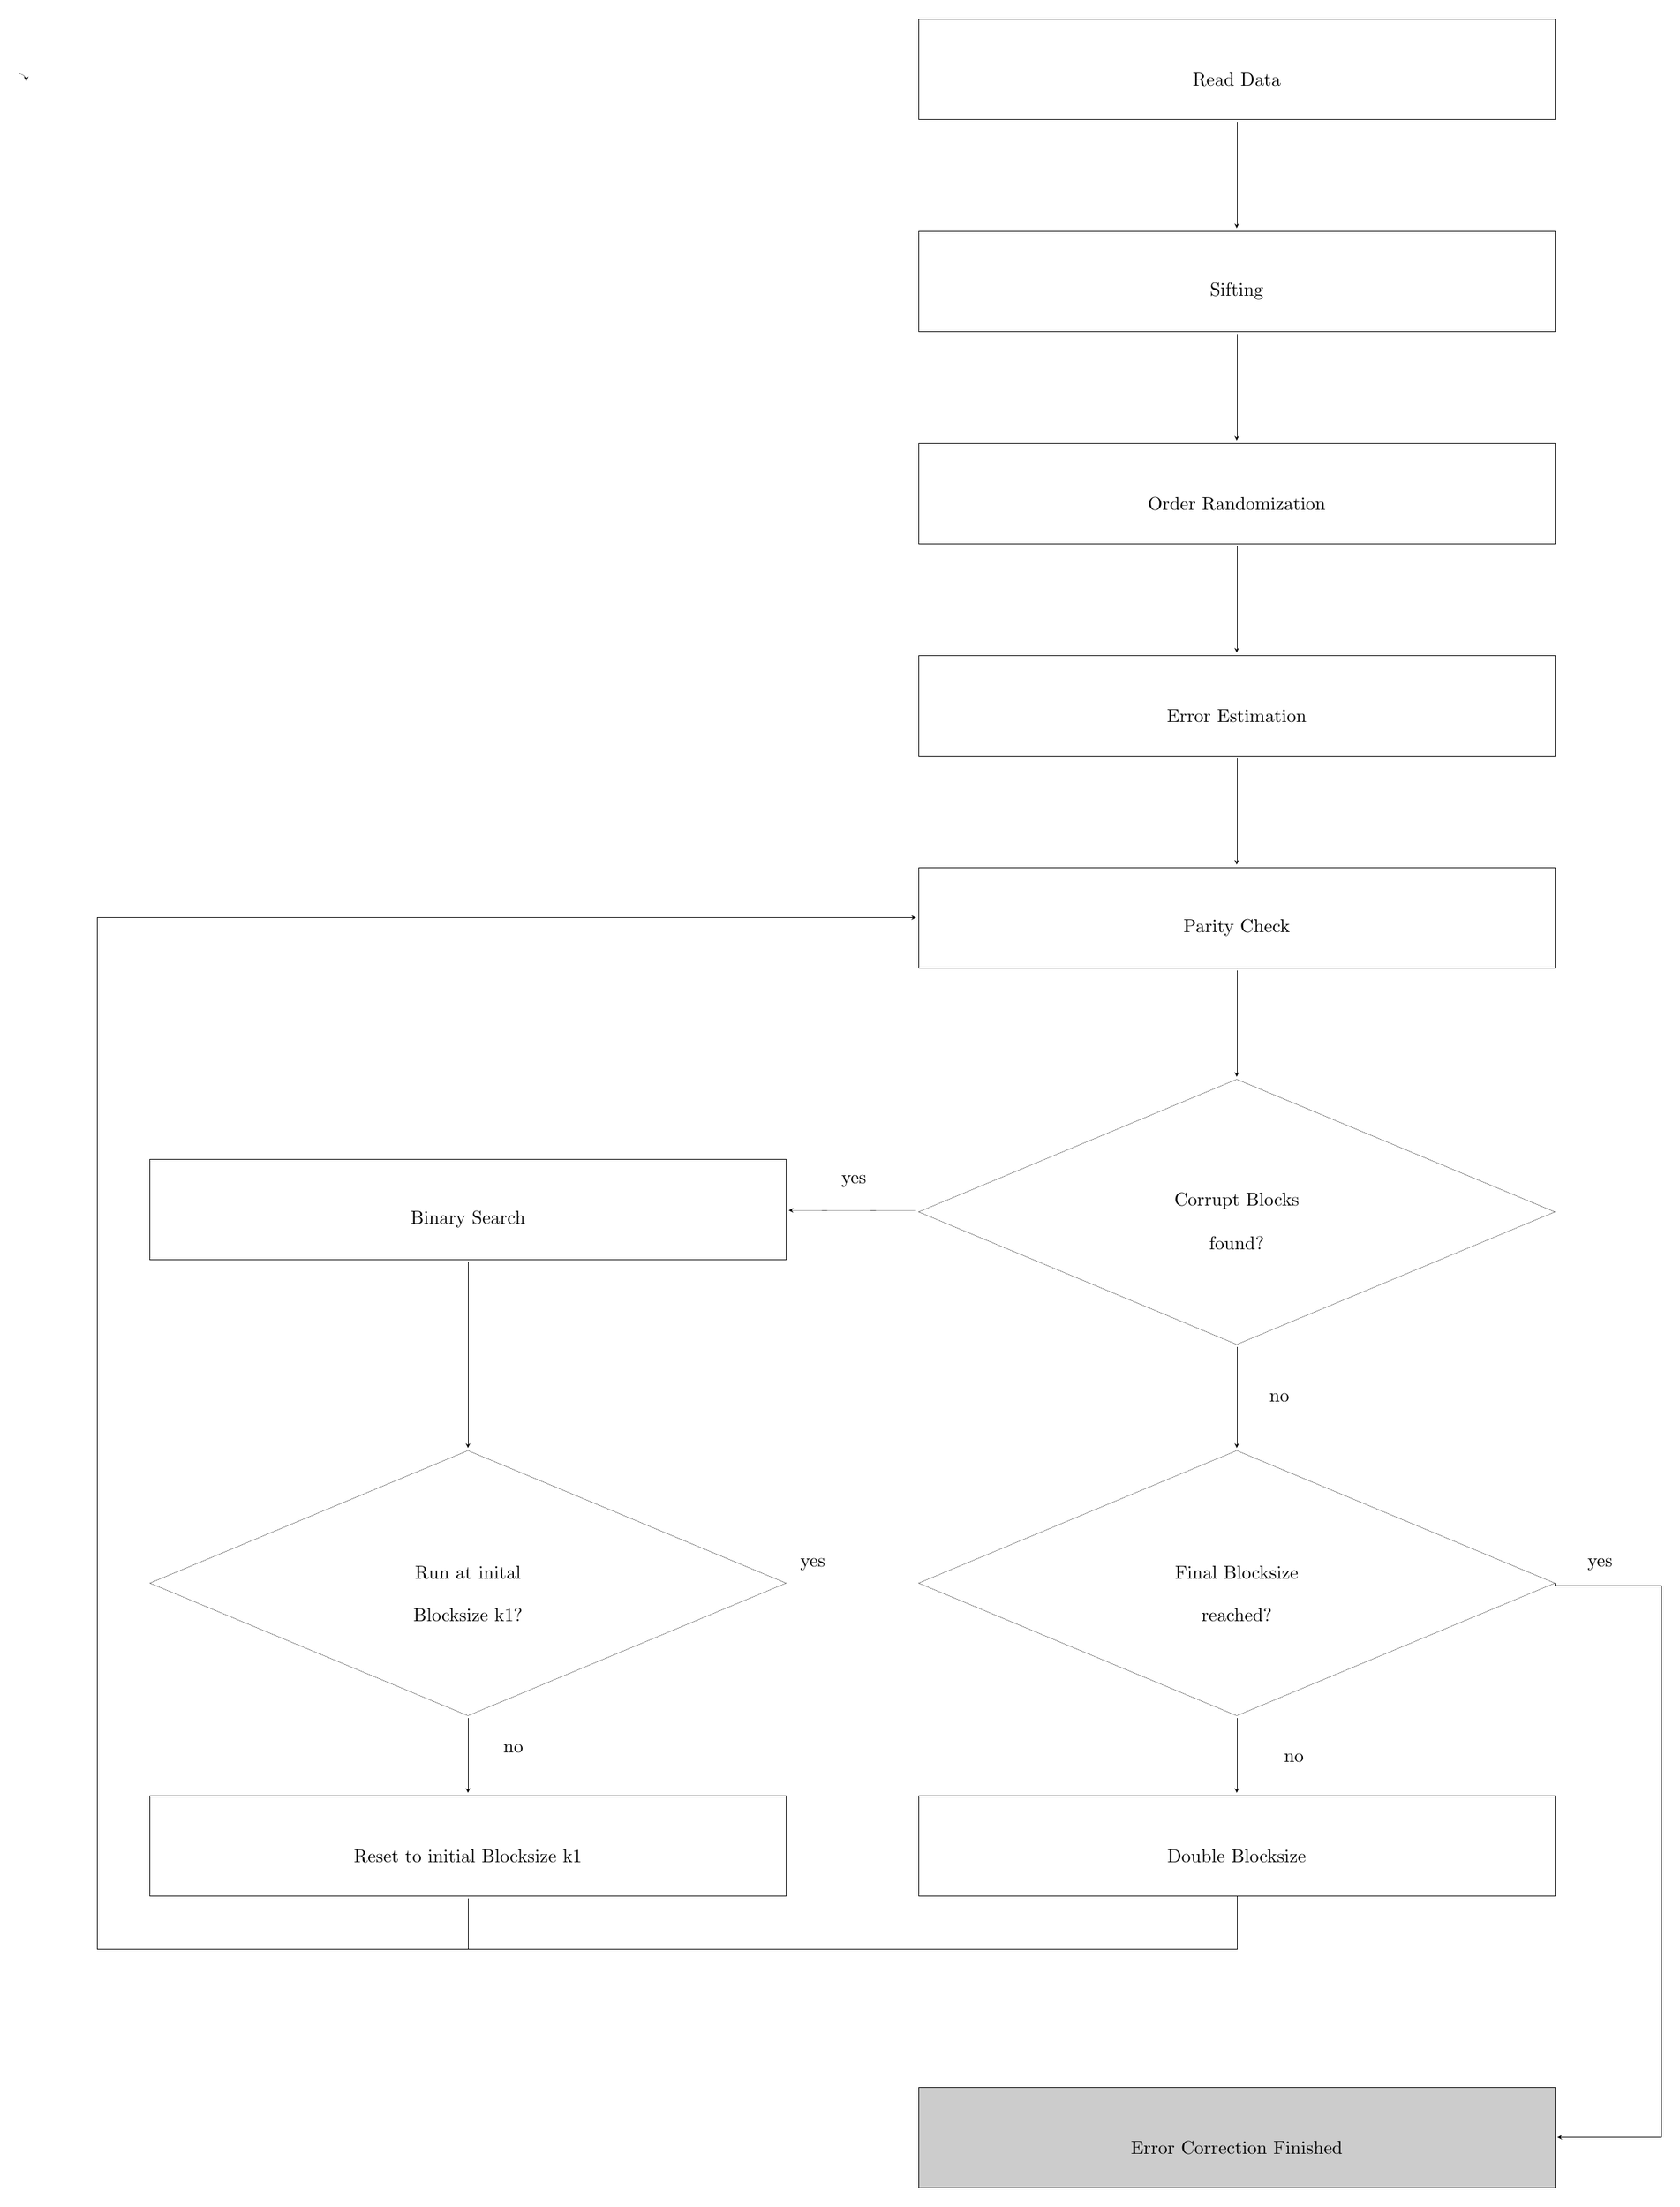
\begin{tikzpicture}
\pgftransformxscale{1.000000}
\pgftransformyscale{-1.000000}
\definecolor{dialinecolor}{rgb}{0.000000, 0.000000, 0.000000}
\pgfsetstrokecolor{dialinecolor}
\definecolor{dialinecolor}{rgb}{1.000000, 1.000000, 1.000000}
\pgfsetfillcolor{dialinecolor}
\definecolor{dialinecolor}{rgb}{1.000000, 1.000000, 1.000000}
\pgfsetfillcolor{dialinecolor}
\fill (17.500000\du,4.000000\du)--(17.500000\du,5.900000\du)--(29.500000\du,5.900000\du)--(29.500000\du,4.000000\du)--cycle;
\pgfsetlinewidth{0.100000\du}
\pgfsetdash{}{0pt}
\pgfsetdash{}{0pt}
\pgfsetmiterjoin
\definecolor{dialinecolor}{rgb}{0.000000, 0.000000, 0.000000}
\pgfsetstrokecolor{dialinecolor}
\draw (17.500000\du,4.000000\du)--(17.500000\du,5.900000\du)--(29.500000\du,5.900000\du)--(29.500000\du,4.000000\du)--cycle;
% setfont left to latex
\definecolor{dialinecolor}{rgb}{0.000000, 0.000000, 0.000000}
\pgfsetstrokecolor{dialinecolor}
\node at (23.500000\du,5.145000\du){Sifting};
\definecolor{dialinecolor}{rgb}{1.000000, 1.000000, 1.000000}
\pgfsetfillcolor{dialinecolor}
\fill (17.500000\du,8.000000\du)--(17.500000\du,9.900000\du)--(29.500000\du,9.900000\du)--(29.500000\du,8.000000\du)--cycle;
\pgfsetlinewidth{0.100000\du}
\pgfsetdash{}{0pt}
\pgfsetdash{}{0pt}
\pgfsetmiterjoin
\definecolor{dialinecolor}{rgb}{0.000000, 0.000000, 0.000000}
\pgfsetstrokecolor{dialinecolor}
\draw (17.500000\du,8.000000\du)--(17.500000\du,9.900000\du)--(29.500000\du,9.900000\du)--(29.500000\du,8.000000\du)--cycle;
% setfont left to latex
\definecolor{dialinecolor}{rgb}{0.000000, 0.000000, 0.000000}
\pgfsetstrokecolor{dialinecolor}
\node at (23.500000\du,9.145000\du){Order Randomization};
\definecolor{dialinecolor}{rgb}{1.000000, 1.000000, 1.000000}
\pgfsetfillcolor{dialinecolor}
\fill (17.500000\du,0.000000\du)--(17.500000\du,1.900000\du)--(29.500000\du,1.900000\du)--(29.500000\du,0.000000\du)--cycle;
\pgfsetlinewidth{0.100000\du}
\pgfsetdash{}{0pt}
\pgfsetdash{}{0pt}
\pgfsetmiterjoin
\definecolor{dialinecolor}{rgb}{0.000000, 0.000000, 0.000000}
\pgfsetstrokecolor{dialinecolor}
\draw (17.500000\du,0.000000\du)--(17.500000\du,1.900000\du)--(29.500000\du,1.900000\du)--(29.500000\du,0.000000\du)--cycle;
% setfont left to latex
\definecolor{dialinecolor}{rgb}{0.000000, 0.000000, 0.000000}
\pgfsetstrokecolor{dialinecolor}
\node at (23.500000\du,1.145000\du){Read Data};
\definecolor{dialinecolor}{rgb}{1.000000, 1.000000, 1.000000}
\pgfsetfillcolor{dialinecolor}
\fill (17.500000\du,16.000000\du)--(17.500000\du,17.900000\du)--(29.500000\du,17.900000\du)--(29.500000\du,16.000000\du)--cycle;
\pgfsetlinewidth{0.100000\du}
\pgfsetdash{}{0pt}
\pgfsetdash{}{0pt}
\pgfsetmiterjoin
\definecolor{dialinecolor}{rgb}{0.000000, 0.000000, 0.000000}
\pgfsetstrokecolor{dialinecolor}
\draw (17.500000\du,16.000000\du)--(17.500000\du,17.900000\du)--(29.500000\du,17.900000\du)--(29.500000\du,16.000000\du)--cycle;
% setfont left to latex
\definecolor{dialinecolor}{rgb}{0.000000, 0.000000, 0.000000}
\pgfsetstrokecolor{dialinecolor}
\node at (23.500000\du,17.145000\du){Parity Check};
\definecolor{dialinecolor}{rgb}{1.000000, 1.000000, 1.000000}
\pgfsetfillcolor{dialinecolor}
\fill (17.500000\du,12.000000\du)--(17.500000\du,13.900000\du)--(29.500000\du,13.900000\du)--(29.500000\du,12.000000\du)--cycle;
\pgfsetlinewidth{0.100000\du}
\pgfsetdash{}{0pt}
\pgfsetdash{}{0pt}
\pgfsetmiterjoin
\definecolor{dialinecolor}{rgb}{0.000000, 0.000000, 0.000000}
\pgfsetstrokecolor{dialinecolor}
\draw (17.500000\du,12.000000\du)--(17.500000\du,13.900000\du)--(29.500000\du,13.900000\du)--(29.500000\du,12.000000\du)--cycle;
% setfont left to latex
\definecolor{dialinecolor}{rgb}{0.000000, 0.000000, 0.000000}
\pgfsetstrokecolor{dialinecolor}
\node at (23.500000\du,13.145000\du){Error Estimation};
\pgfsetlinewidth{0.100000\du}
\pgfsetdash{}{0pt}
\pgfsetdash{}{0pt}
\pgfsetbuttcap
{
\definecolor{dialinecolor}{rgb}{0.000000, 0.000000, 0.000000}
\pgfsetfillcolor{dialinecolor}
% was here!!!
\pgfsetarrowsend{stealth}
\definecolor{dialinecolor}{rgb}{0.000000, 0.000000, 0.000000}
\pgfsetstrokecolor{dialinecolor}
\draw (23.500000\du,1.950488\du)--(23.500000\du,3.949512\du);
}
\pgfsetlinewidth{0.100000\du}
\pgfsetdash{}{0pt}
\pgfsetdash{}{0pt}
\pgfsetbuttcap
{
\definecolor{dialinecolor}{rgb}{0.000000, 0.000000, 0.000000}
\pgfsetfillcolor{dialinecolor}
% was here!!!
\pgfsetarrowsend{stealth}
\definecolor{dialinecolor}{rgb}{0.000000, 0.000000, 0.000000}
\pgfsetstrokecolor{dialinecolor}
\draw (23.500000\du,5.950488\du)--(23.500000\du,7.949512\du);
}
\pgfsetlinewidth{0.100000\du}
\pgfsetdash{}{0pt}
\pgfsetdash{}{0pt}
\pgfsetbuttcap
{
\definecolor{dialinecolor}{rgb}{0.000000, 0.000000, 0.000000}
\pgfsetfillcolor{dialinecolor}
% was here!!!
\pgfsetarrowsend{stealth}
\definecolor{dialinecolor}{rgb}{0.000000, 0.000000, 0.000000}
\pgfsetstrokecolor{dialinecolor}
\draw (23.500000\du,9.950488\du)--(23.500000\du,11.949512\du);
}
\pgfsetlinewidth{0.100000\du}
\pgfsetdash{}{0pt}
\pgfsetdash{}{0pt}
\pgfsetbuttcap
{
\definecolor{dialinecolor}{rgb}{0.000000, 0.000000, 0.000000}
\pgfsetfillcolor{dialinecolor}
% was here!!!
\pgfsetarrowsend{stealth}
\definecolor{dialinecolor}{rgb}{0.000000, 0.000000, 0.000000}
\pgfsetstrokecolor{dialinecolor}
\draw (23.500000\du,13.950488\du)--(23.500000\du,15.949512\du);
}
\definecolor{dialinecolor}{rgb}{1.000000, 1.000000, 1.000000}
\pgfsetfillcolor{dialinecolor}
\fill (23.500000\du,20.000000\du)--(29.500000\du,22.500000\du)--(23.500000\du,25.000000\du)--(17.500000\du,22.500000\du)--cycle;
\pgfsetlinewidth{0.100000\du}
\pgfsetdash{}{0pt}
\pgfsetdash{}{0pt}
\pgfsetmiterjoin
\definecolor{dialinecolor}{rgb}{0.000000, 0.000000, 0.000000}
\pgfsetstrokecolor{dialinecolor}
\draw (23.500000\du,20.000000\du)--(29.500000\du,22.500000\du)--(23.500000\du,25.000000\du)--(17.500000\du,22.500000\du)--cycle;
% setfont left to latex
\definecolor{dialinecolor}{rgb}{0.000000, 0.000000, 0.000000}
\pgfsetstrokecolor{dialinecolor}
\node at (23.500000\du,22.295000\du){Corrupt Blocks};
% setfont left to latex
\definecolor{dialinecolor}{rgb}{0.000000, 0.000000, 0.000000}
\pgfsetstrokecolor{dialinecolor}
\node at (23.500000\du,23.095000\du){found?};
\pgfsetlinewidth{0.100000\du}
\pgfsetdash{}{0pt}
\pgfsetdash{}{0pt}
\pgfsetbuttcap
{
\definecolor{dialinecolor}{rgb}{0.000000, 0.000000, 0.000000}
\pgfsetfillcolor{dialinecolor}
% was here!!!
\pgfsetarrowsend{stealth}
\definecolor{dialinecolor}{rgb}{0.000000, 0.000000, 0.000000}
\pgfsetstrokecolor{dialinecolor}
\draw (23.500000\du,17.950314\du)--(23.500000\du,19.950000\du);
}
\definecolor{dialinecolor}{rgb}{1.000000, 1.000000, 1.000000}
\pgfsetfillcolor{dialinecolor}
\fill (3.000000\du,21.500000\du)--(3.000000\du,23.400000\du)--(15.000000\du,23.400000\du)--(15.000000\du,21.500000\du)--cycle;
\pgfsetlinewidth{0.100000\du}
\pgfsetdash{}{0pt}
\pgfsetdash{}{0pt}
\pgfsetmiterjoin
\definecolor{dialinecolor}{rgb}{0.000000, 0.000000, 0.000000}
\pgfsetstrokecolor{dialinecolor}
\draw (3.000000\du,21.500000\du)--(3.000000\du,23.400000\du)--(15.000000\du,23.400000\du)--(15.000000\du,21.500000\du)--cycle;
% setfont left to latex
\definecolor{dialinecolor}{rgb}{0.000000, 0.000000, 0.000000}
\pgfsetstrokecolor{dialinecolor}
\node at (9.000000\du,22.645000\du){Binary Search};
\definecolor{dialinecolor}{rgb}{1.000000, 1.000000, 1.000000}
\pgfsetfillcolor{dialinecolor}
\fill (9.000000\du,27.000000\du)--(15.000000\du,29.500000\du)--(9.000000\du,32.000000\du)--(3.000000\du,29.500000\du)--cycle;
\pgfsetlinewidth{0.100000\du}
\pgfsetdash{}{0pt}
\pgfsetdash{}{0pt}
\pgfsetmiterjoin
\definecolor{dialinecolor}{rgb}{0.000000, 0.000000, 0.000000}
\pgfsetstrokecolor{dialinecolor}
\draw (9.000000\du,27.000000\du)--(15.000000\du,29.500000\du)--(9.000000\du,32.000000\du)--(3.000000\du,29.500000\du)--cycle;
% setfont left to latex
\definecolor{dialinecolor}{rgb}{0.000000, 0.000000, 0.000000}
\pgfsetstrokecolor{dialinecolor}
\node at (9.000000\du,29.295000\du){Run at inital};
% setfont left to latex
\definecolor{dialinecolor}{rgb}{0.000000, 0.000000, 0.000000}
\pgfsetstrokecolor{dialinecolor}
\node at (9.000000\du,30.095000\du){Blocksize k1?};
\pgfsetlinewidth{0.100000\du}
\pgfsetdash{}{0pt}
\pgfsetdash{}{0pt}
\pgfsetbuttcap
{
\definecolor{dialinecolor}{rgb}{0.000000, 0.000000, 0.000000}
\pgfsetfillcolor{dialinecolor}
% was here!!!
\pgfsetarrowsend{stealth}
\definecolor{dialinecolor}{rgb}{0.000000, 0.000000, 0.000000}
\pgfsetstrokecolor{dialinecolor}
\draw (17.450000\du,22.479138\du)--(15.050369\du,22.470863\du);
}
\pgfsetlinewidth{0.100000\du}
\pgfsetdash{}{0pt}
\pgfsetdash{}{0pt}
\pgfsetbuttcap
{
\definecolor{dialinecolor}{rgb}{0.000000, 0.000000, 0.000000}
\pgfsetfillcolor{dialinecolor}
% was here!!!
\pgfsetarrowsend{stealth}
\definecolor{dialinecolor}{rgb}{0.000000, 0.000000, 0.000000}
\pgfsetstrokecolor{dialinecolor}
\draw (9.000000\du,23.449152\du)--(9.000000\du,26.950000\du);
}
\definecolor{dialinecolor}{rgb}{1.000000, 1.000000, 1.000000}
\pgfsetfillcolor{dialinecolor}
\fill (3.000000\du,33.500000\du)--(3.000000\du,35.400000\du)--(15.000000\du,35.400000\du)--(15.000000\du,33.500000\du)--cycle;
\pgfsetlinewidth{0.100000\du}
\pgfsetdash{}{0pt}
\pgfsetdash{}{0pt}
\pgfsetmiterjoin
\definecolor{dialinecolor}{rgb}{0.000000, 0.000000, 0.000000}
\pgfsetstrokecolor{dialinecolor}
\draw (3.000000\du,33.500000\du)--(3.000000\du,35.400000\du)--(15.000000\du,35.400000\du)--(15.000000\du,33.500000\du)--cycle;
% setfont left to latex
\definecolor{dialinecolor}{rgb}{0.000000, 0.000000, 0.000000}
\pgfsetstrokecolor{dialinecolor}
\node at (9.000000\du,34.645000\du){Reset to initial Blocksize k1};
\pgfsetlinewidth{0.100000\du}
\pgfsetdash{}{0pt}
\pgfsetdash{}{0pt}
\pgfsetbuttcap
{
\definecolor{dialinecolor}{rgb}{0.000000, 0.000000, 0.000000}
\pgfsetfillcolor{dialinecolor}
% was here!!!
\pgfsetarrowsend{stealth}
\definecolor{dialinecolor}{rgb}{0.000000, 0.000000, 0.000000}
\pgfsetstrokecolor{dialinecolor}
\draw (9.000000\du,32.050000\du)--(9.000000\du,33.451782\du);
}
\definecolor{dialinecolor}{rgb}{1.000000, 1.000000, 1.000000}
\pgfsetfillcolor{dialinecolor}
\fill (17.500000\du,33.500000\du)--(17.500000\du,35.400000\du)--(29.500000\du,35.400000\du)--(29.500000\du,33.500000\du)--cycle;
\pgfsetlinewidth{0.100000\du}
\pgfsetdash{}{0pt}
\pgfsetdash{}{0pt}
\pgfsetmiterjoin
\definecolor{dialinecolor}{rgb}{0.000000, 0.000000, 0.000000}
\pgfsetstrokecolor{dialinecolor}
\draw (17.500000\du,33.500000\du)--(17.500000\du,35.400000\du)--(29.500000\du,35.400000\du)--(29.500000\du,33.500000\du)--cycle;
% setfont left to latex
\definecolor{dialinecolor}{rgb}{0.000000, 0.000000, 0.000000}
\pgfsetstrokecolor{dialinecolor}
\node at (23.500000\du,34.645000\du){Double Blocksize};
\definecolor{dialinecolor}{rgb}{1.000000, 1.000000, 1.000000}
\pgfsetfillcolor{dialinecolor}
\fill (23.500000\du,27.000000\du)--(29.500000\du,29.500000\du)--(23.500000\du,32.000000\du)--(17.500000\du,29.500000\du)--cycle;
\pgfsetlinewidth{0.100000\du}
\pgfsetdash{}{0pt}
\pgfsetdash{}{0pt}
\pgfsetmiterjoin
\definecolor{dialinecolor}{rgb}{0.000000, 0.000000, 0.000000}
\pgfsetstrokecolor{dialinecolor}
\draw (23.500000\du,27.000000\du)--(29.500000\du,29.500000\du)--(23.500000\du,32.000000\du)--(17.500000\du,29.500000\du)--cycle;
% setfont left to latex
\definecolor{dialinecolor}{rgb}{0.000000, 0.000000, 0.000000}
\pgfsetstrokecolor{dialinecolor}
\node at (23.500000\du,29.295000\du){Final Blocksize};
% setfont left to latex
\definecolor{dialinecolor}{rgb}{0.000000, 0.000000, 0.000000}
\pgfsetstrokecolor{dialinecolor}
\node at (23.500000\du,30.095000\du){reached?};
\pgfsetlinewidth{0.100000\du}
\pgfsetdash{}{0pt}
\pgfsetdash{}{0pt}
\pgfsetbuttcap
{
\definecolor{dialinecolor}{rgb}{0.000000, 0.000000, 0.000000}
\pgfsetfillcolor{dialinecolor}
% was here!!!
\pgfsetarrowsend{stealth}
\definecolor{dialinecolor}{rgb}{0.000000, 0.000000, 0.000000}
\pgfsetstrokecolor{dialinecolor}
\draw (23.500000\du,25.050000\du)--(23.500000\du,26.950000\du);
}
\definecolor{dialinecolor}{rgb}{0.800000, 0.800000, 0.800000}
\pgfsetfillcolor{dialinecolor}
\fill (17.500000\du,39.000000\du)--(17.500000\du,40.900000\du)--(29.500000\du,40.900000\du)--(29.500000\du,39.000000\du)--cycle;
\pgfsetlinewidth{0.100000\du}
\pgfsetdash{}{0pt}
\pgfsetdash{}{0pt}
\pgfsetmiterjoin
\definecolor{dialinecolor}{rgb}{0.000000, 0.000000, 0.000000}
\pgfsetstrokecolor{dialinecolor}
\draw (17.500000\du,39.000000\du)--(17.500000\du,40.900000\du)--(29.500000\du,40.900000\du)--(29.500000\du,39.000000\du)--cycle;
% setfont left to latex
\definecolor{dialinecolor}{rgb}{0.000000, 0.000000, 0.000000}
\pgfsetstrokecolor{dialinecolor}
\node at (23.500000\du,40.145000\du){Error Correction Finished};
\pgfsetlinewidth{0.100000\du}
\pgfsetdash{}{0pt}
\pgfsetdash{}{0pt}
\pgfsetbuttcap
{
\definecolor{dialinecolor}{rgb}{0.000000, 0.000000, 0.000000}
\pgfsetfillcolor{dialinecolor}
% was here!!!
\pgfsetarrowsend{stealth}
\definecolor{dialinecolor}{rgb}{0.000000, 0.000000, 0.000000}
\pgfsetstrokecolor{dialinecolor}
\draw (23.500000\du,32.050000\du)--(23.500000\du,33.451782\du);
}
\pgfsetlinewidth{0.100000\du}
\pgfsetdash{}{0pt}
\pgfsetdash{}{0pt}
\pgfsetmiterjoin
\pgfsetbuttcap
{
\definecolor{dialinecolor}{rgb}{0.000000, 0.000000, 0.000000}
\pgfsetfillcolor{dialinecolor}
% was here!!!
\pgfsetarrowsend{stealth}
\definecolor{dialinecolor}{rgb}{0.000000, 0.000000, 0.000000}
\pgfsetstrokecolor{dialinecolor}
\pgfpathmoveto{\pgfpoint{15.000000\du}{29.500000\du}}
\pgfpathcurveto{\pgfpoint{17.822000\du}{29.500000\du}}{\pgfpoint{19.000000\du}{32.000000\du}}{\pgfpoint{19.000000\du}{33.500000\du}}
\pgfusepath{stroke}
}
\pgfsetlinewidth{0.100000\du}
\pgfsetdash{}{0pt}
\pgfsetdash{}{0pt}
\pgfsetmiterjoin
\pgfsetbuttcap
{
\definecolor{dialinecolor}{rgb}{0.000000, 0.000000, 0.000000}
\pgfsetfillcolor{dialinecolor}
% was here!!!
\pgfsetarrowsend{stealth}
{\pgfsetcornersarced{\pgfpoint{0.000000\du}{0.000000\du}}\definecolor{dialinecolor}{rgb}{0.000000, 0.000000, 0.000000}
\pgfsetstrokecolor{dialinecolor}
\draw (23.500000\du,35.400000\du)--(23.500000\du,36.400000\du)--(2.000000\du,36.400000\du)--(2.000000\du,16.950000\du)--(17.449844\du,16.950000\du);
}}
\pgfsetlinewidth{0.100000\du}
\pgfsetdash{}{0pt}
\pgfsetdash{}{0pt}
\pgfsetbuttcap
{
\definecolor{dialinecolor}{rgb}{0.000000, 0.000000, 0.000000}
\pgfsetfillcolor{dialinecolor}
% was here!!!
\definecolor{dialinecolor}{rgb}{0.000000, 0.000000, 0.000000}
\pgfsetstrokecolor{dialinecolor}
\draw (9.000000\du,35.450232\du)--(9.000000\du,36.400000\du);
}
% setfont left to latex
\definecolor{dialinecolor}{rgb}{0.000000, 0.000000, 0.000000}
\pgfsetstrokecolor{dialinecolor}
\node[anchor=west] at (15.925000\du,21.925000\du){yes};
% setfont left to latex
\definecolor{dialinecolor}{rgb}{0.000000, 0.000000, 0.000000}
\pgfsetstrokecolor{dialinecolor}
\node[anchor=west] at (24.000000\du,26.000000\du){no};
% setfont left to latex
\definecolor{dialinecolor}{rgb}{0.000000, 0.000000, 0.000000}
\pgfsetstrokecolor{dialinecolor}
\node[anchor=west] at (15.150000\du,29.150000\du){yes};
% setfont left to latex
\definecolor{dialinecolor}{rgb}{0.000000, 0.000000, 0.000000}
\pgfsetstrokecolor{dialinecolor}
\node[anchor=west] at (9.550000\du,32.625000\du){no};
% setfont left to latex
\definecolor{dialinecolor}{rgb}{0.000000, 0.000000, 0.000000}
\pgfsetstrokecolor{dialinecolor}
\node[anchor=west] at (24.275000\du,32.800000\du){no};
% setfont left to latex
\definecolor{dialinecolor}{rgb}{0.000000, 0.000000, 0.000000}
\pgfsetstrokecolor{dialinecolor}
\node[anchor=west] at (30.000000\du,29.150000\du){yes};
\pgfsetlinewidth{0.100000\du}
\pgfsetdash{}{0pt}
\pgfsetdash{}{0pt}
\pgfsetmiterjoin
\pgfsetbuttcap
{
\definecolor{dialinecolor}{rgb}{0.000000, 0.000000, 0.000000}
\pgfsetfillcolor{dialinecolor}
% was here!!!
\pgfsetarrowsend{stealth}
{\pgfsetcornersarced{\pgfpoint{0.000000\du}{0.000000\du}}\definecolor{dialinecolor}{rgb}{0.000000, 0.000000, 0.000000}
\pgfsetstrokecolor{dialinecolor}
\draw (29.500000\du,29.500000\du)--(29.500000\du,29.550000\du)--(31.500000\du,29.550000\du)--(31.500000\du,39.950000\du)--(29.548828\du,39.950000\du);
}}
\end{tikzpicture}

\caption{Float Diagram for Error Correction}
\end{figure}


\end{document}